\documentclass[12pt,
article,
type=prosem, %sta, diplom, bsc, pp, msc, dr, drfinal, sem, prosem, bsc
colorbacktitle,
instlogo,
accentcolor=tud1c,
%twoside
]{tudthesis}

\usepackage[ngerman]{babel}
%\usepackage[english]{babel}

\usepackage[T1]{fontenc}
\usepackage[utf8]{inputenc}
%\usepackage[applemac]{inputenc}

% linebreak for urls in bitex
\usepackage{url}
\urlstyle{rm}

%listings
\usepackage{listings}
\usepackage{xcolor}
\lstset { %
	language=C++,
	backgroundcolor=\color{black!5}, % set backgroundcolor
	basicstyle=\footnotesize,% basic font setting
}

\newcommand{\getmydate}{%
\iflanguage{ngerman}{%
  \ifcase\month%
    \or Januar\or Februar\or M\"arz%
    \or April\or Mai\or Juni\or Juli%
    \or August\or September\or Oktober%
    \or November\or Dezember%
  \fi\ \number\year%
}%
\iflanguage{english}{%
  \ifcase\month%
    \or January\or February\or March%
    \or April\or May\or June\or July%
    \or August\or September\or October%
    \or November\or December%
  \fi\ \number\year%
}
}
% changed counter for section wise counting
\usepackage{chngcntr}
\counterwithin{figure}{section} 
\counterwithin{table}{section} 

 
\setinstitutionlogo[height]{logo/ESlogo.png}

\begin{document}
	\counterwithin{lstlisting}{section}
  \thesistitle{Projektseminar Echtzeitsysteme}%
    {Ausarbeitung von Team TRAL}
  \author{Tim Burkert, Robert Königstein, Lars Stein, Adrian Weber}
  %do not add your student id!
  %\studentidx{1145456}
	\thesisnumber{ES-B-0060}
  \referee{Prof. Dr. rer. nat. A. Schürr}{Géza Kulcsar}
	
  \iflanguage{english}{
		\department{	\mbox{Department of Electrical Engineering}\\ and Information Technology (FB18)\\\\Adjunct Member Department of\\ Computer Science (FB20)\\\\Prof. Dr. rer. nat. A. Schürr\\\ Merckstraße 25\\64283 Darmstadt\\\\www.es.tu-darmstadt.de}
		\group{Real-Time Systems Lab}
	}{
		\department{Elektrotechnik und \\Informationstechnik (FB18)\\\\Zweitmitglied Informatik (FB20)\\\\Prof. Dr. rer. nat. A. Schürr\\\ Merckstraße 25\\64283 Darmstadt\\\\www.es.tu-darmstadt.de}
		\group{Fachgebiet Echtzeitsysteme}
	}
  
  \dateofsubmit{\today}
  \makethesistitle
  \affidavit{Adrian Weber, Tim Burkert, Lars Stein, Robert Königstein}
	
	%\cleardoublepage
	
	%%% Zusammenfassung vor Inhaltsverzeichnis
	%\begin {abstract}
	%...hallo
	%\end{abstract} 
	
	\cleardoublepage
	

	\pagenumbering{roman}
	\addtocontents{Anhang}{}
	\tableofcontents
	\cleardoublepage
	\listoffigures
	\cleardoublepage
	\listoftables
	\cleardoublepage
	
	\pagenumbering{arabic}
	
	%%% Hier stehen alle von uns eingebundenen Kapitel	
	\section{Einleitung}
\label{sec:einleitung}
\subsection{Motivation}
Die Themengebiete Fahrassistenzsysteme und vor allem autonomes Fahren sind heute aktueller denn je. Zum einen, da vieles längst keine Zukunftsmusik mehr darstellt und schon in unserem alltäglichen Leben angekommen ist. Hierzu zählen Systeme zur Überwachung toter Winkel, vom elektrischen Spiegel bis hin zur Rundumsicht im Bird-View-System. Nicht nur Warnsysteme, die den Fahrer auf gefährliche Situationen hinweisen, sondern auch halbautomatische Piloten, die korrigierend eingreifen, sind Realität. Beispiele hierfür sind Lenk- und Parkassistenten, wie auch automatische Notbremssysteme, die nicht nur statische Hindernisse erkennen, sondern sogar die Bewegung kreuzender Autos vorausberechnen können. Hierbei scheint sogar oftmals nicht die Technik, sondern die Rechtslage das begrenzende Element darzustellen.
\newline
Zum anderen, da mit jeder weiteren Funktionalität die Gesamtkomplexität eines möglicherweise autonom fahrenden Fahrzeugs noch deutlicher vor Augen geführt wird. Es werden weitere Probleme erkannt, die beachtet und absolut zuverlässig gelöst werden müssen, da im Falle eines Ausfalls oder Fehlverhaltens des Systems Menschenleben auf dem Spiel stehen. Um eine Situation vollständig zu erkennen und korrekt auszuwerten, ist die Zusammenarbeit mehrerer unterschiedlicher Sensoren nötig. So werden Autos mit (Stereo-) Kameras, Ultraschall und sogar Radar ausgestattet, um auf unterschiedliche Distanz und Richtung Aussagen über die Umgebung machen zu können. Dabei müssen natürlich alle Berechnungen vor Ort und in Echtzeit durchgeführt werden.

%%%%%%%%%%
\subsection{Das Projektseminar Echtzeitsysteme}
Bereits seit einigen Jahren bietet daher das Fachgebiet Echtzeitsysteme das gleichnamige Projektseminar an. Schwerpunkte waren dabei stets (halb-) autonomes Fahren und Car2X Kommunikation. Realisiert wurde dies mittels eines bzw. mehrerer Modellauto-Chassis mit Motoren und Sensoren, gesteuert von einem 16Bit Mikrocontroller. Um den gesteigerten Anforderungen Rechnung zu tragen, wurden erstmalig dieses Semester die Fahrzeuge mit einer weiteren Platine ausgestattet, die aufgrund des verbauten Prozessors komplexere und rechenaufwändigere Aufgaben ermöglichten, so zum Beispiel Videoverarbeitung zusammen mit der ebenfalls neu angebrachten Kamera. So wurde auch das Spektrum der Aufgabenstellung erweitert und erstreckt sich nun von geregeltem Fahren mit Abstandssensoren bis hin zum Anfahren eines Ziels, wobei das Ziel selbstständig mit der Kamera erfasst werden muss. Dabei war die genaue Realisierung der Anforderungen bewusst freigestellt. Auch weitere vertiefende Themen konnten von den Teams selbst ausgewählt werden. Dies ermöglichte ein sehr eigenständiges Arbeiten in der Gruppe, da hier in großem Umfang und für jedes Team individuell, sowohl die Interessen, als auch die Kompetenzen berücksichtigt werden konnten. Ein übergeordneter Gedanke war dabei stets die Nachhaltigkeit, damit die Teams in kommenden Semestern von den Ergebnissen profitieren und im Idealfall darauf aufbauen können. Diese Nachhaltigkeit ist sehr wichtig und stellt auch ein Kernthema unserer Ergebnisse dar. Fernziel des Projektseminars ist nämlich das Erarbeiten einer Plattform, die eine Teilnahme am \textit{Carolo Cup}\footnote[1]{https://wiki.ifr.ing.tu-bs.de/carolocup/} oder ähnlichen Veranstaltungen ermöglicht.

	\cleardoublepage
	\section{Zur Verfügung gestellte Hardware des Autos}
\label{sec:grundlegendesHW}

Die Basis der zur Verfügung stehenden Hardware, also Chassis, Motoren, Servo, etc. sind handelsübliche Modellautos. Dabei besteht das Auto aus zwei Schichten. Die Basis bildet ein 16-Bit Mikrocontroller der MB96300-Serie von \textit{Fujitsu Microelectronics} (heute: \textit{Cypress Semiconductor Corporation}). Die zweite Schicht der Hardware des Autos besteht aus einem vollwertigen Einplatinencomputer mit Quad-Core-Prozessor, SSD-Speicher uvm. Der Mikrokontroller ist in der zu diesem Semester upgegradeten Hardware nur noch zur Vermittlung der Werte von Sensorik und Aktorik zwischen Hauptplatine und Peripherie zuständig. Somit hatten wir eine vollwertige API zur Hardware, sodass keine Software für Schnittstellen oder Treiber implementiert werden musste und (fast) keine Veränderungen am Mikrocontroller vorgenommen werden mussten. Als Sensoren stehen ein Hall-Sensor am Hinterrad, ein Liniensenor, eine USB-Webcam, sowie drei Ultraschallsensoren (rechts, links und vorne) zur Verfügung. Angesteuert wird die Lenkung des Modellautos über einen Servo-Motor. Der Antrieb des Autos ist durch einen Gleichstrommotor, der durch einen Fahrtregler fast stufenlos angesteuert werden kann, realisiert. Beides wird durch ein pulsweitenmoduliertes Signal vom Mikrokontroller gesteuert. Zudem ist ein WLAN-Modul integriert, sodass es möglich ist, auf das Auto per Ad-hoc-Verbindung zuzugreifen. 

\begin{figure}[htbp] 
	\centering
	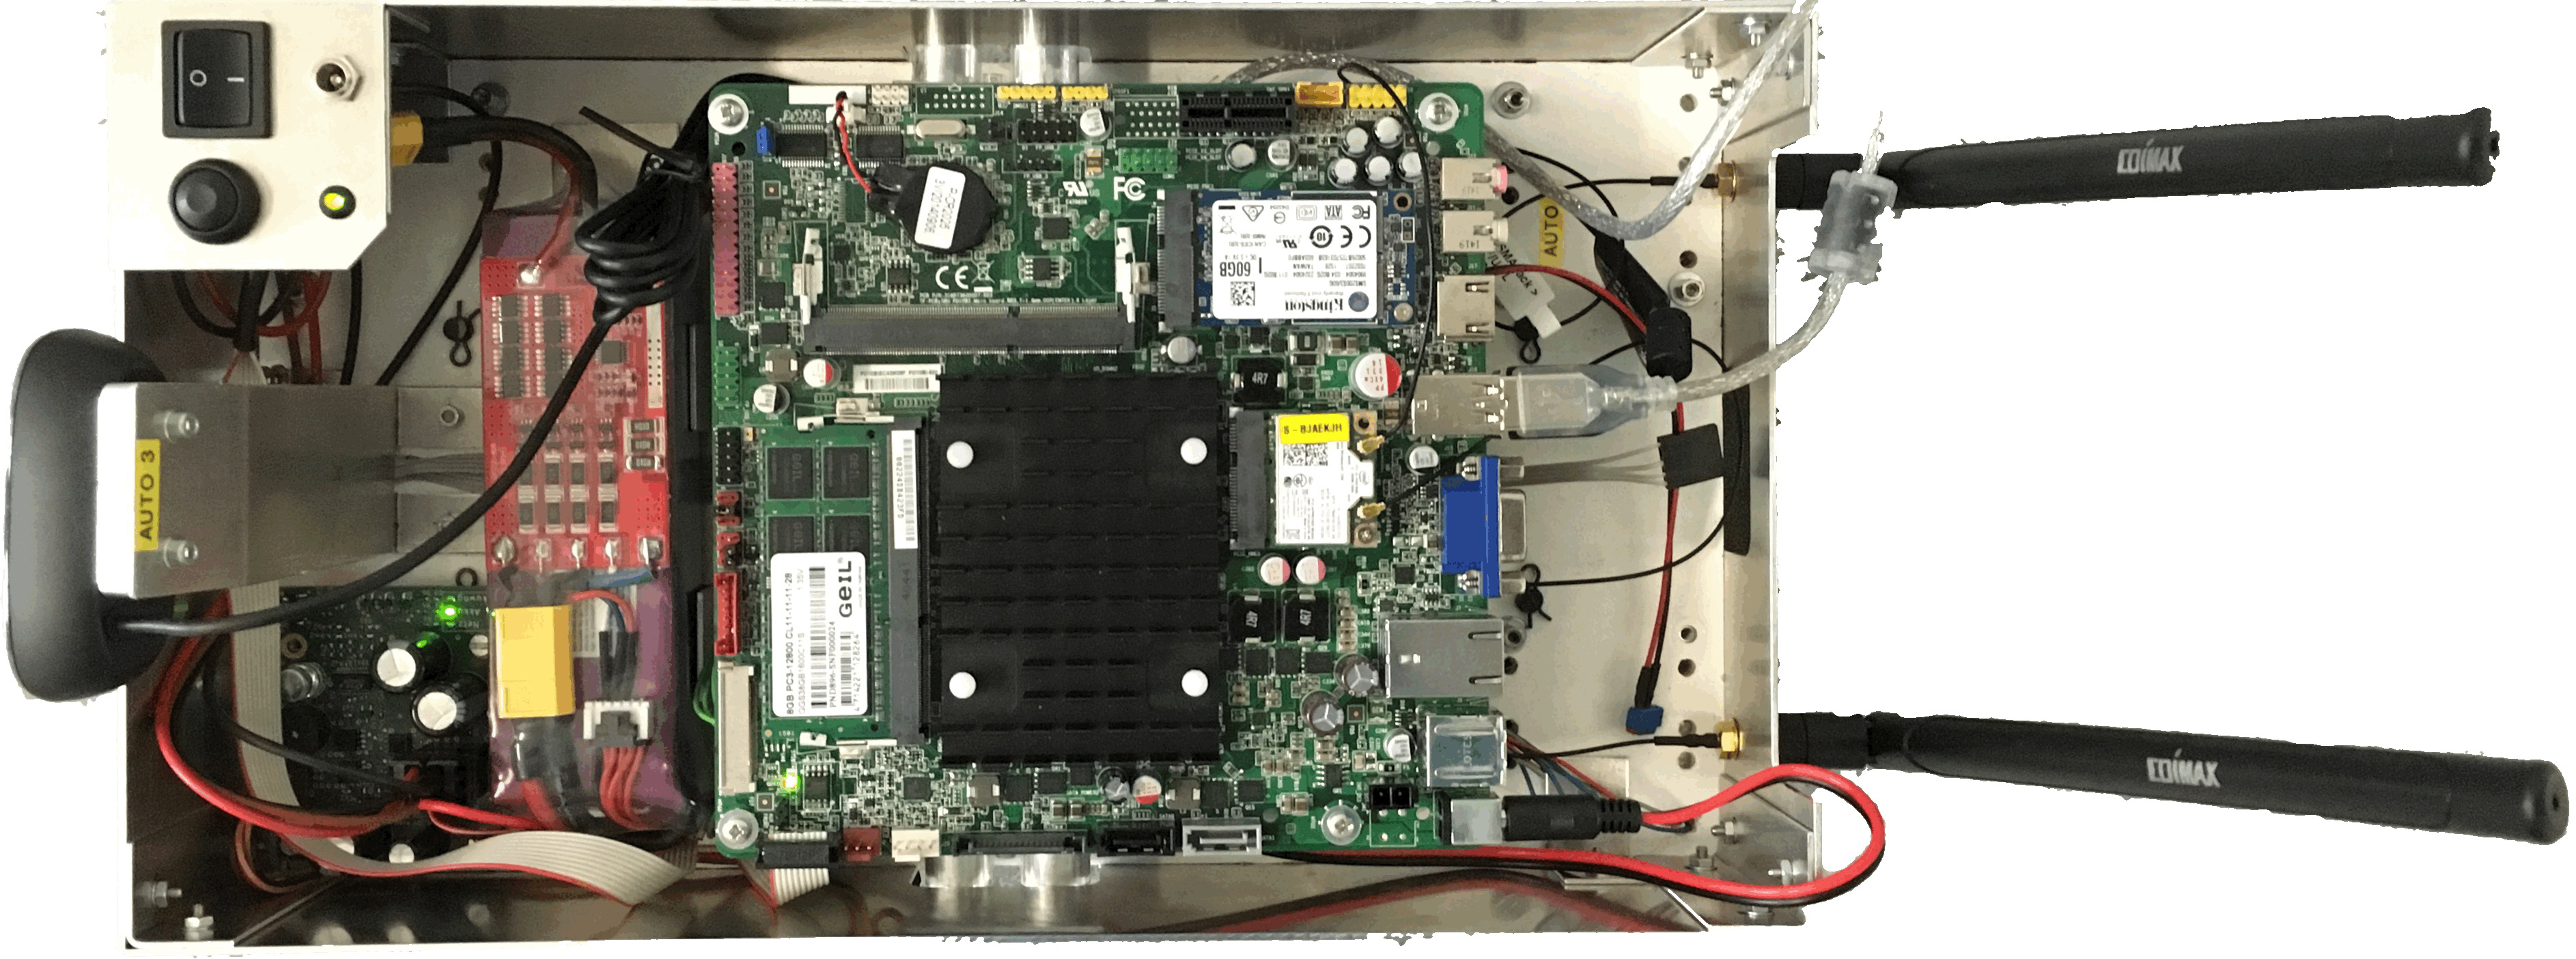
\includegraphics[width=350pt]{images/Animauto.jpg}
	\caption{Das Auto}
	\label{fig:DasAuto}
\end{figure}

Die Software auf dem Mikrokontroller, die zur Kommunikation zwischen der Anwendungssoftware und der Sensorik bzw. Aktorik zuständig ist, ist bereits vorimplementiert. Durch die so zur Verfügung gestellte API war eine einfache Nutzung der Hardware möglich. Jedoch war dadurch auch unklar, inwieweit die Signale der Sensorik manipuliert wurden. Die Ultraschallsensoren waren zu Beginn auf cm-Auflösung eingestellt, was zu ungenauen Sensorwerten führte. Die abbildbare Tiefe betrug etwa 20 cm bis 3 m mit vielen Ausreißern und Diskrepanzen durch eine niedrige Auflösung. Um bessere Werte zu erhalten, haben wir auf dem Mikrokontroller von cm-Werte auf Mikrosekunden-Werte umgestellt. Dies hat die Genauigkeit, sowie den Messbereich erhöht.
	\cleardoublepage
	\section{Grundlegendes zu \textit{ROS} und Lubuntu}
\label{sec:grundlegendesROS-OS}   
Im Folgenden wird eine kurze Einleitung zu ROS und dem Betriebssystem, das auf dem Auto installiert war, Lubuntu, gegeben. Diese Grundausstattung an Software war bei allen Gruppen identisch.
%%%%%%
\subsection{Was ist \textit{ROS}?}
Im Projektseminar wird die Middleware \textit{ROS} eingesetzt. \textit{ROS} steht für \textit{Robot Operating System} und wird heute vor allem von der \textit{Open Source Robotics Foundation} fortentwickelt. Die Software ist dabei kein klassisches Betriebssystem, wie der Name vermuten lässt, sondern eine Middleware, die auf einem der klassischen Betriebssysteme (aktuell werden Mac-OS und Linux stabil unterstützt) aufgespielt wird. \textit{ROS} sorgt für eine starke Hardware-Abstraktion, sodass fast beliebige Hardware eingesetzt werden kann und diese auch fast beliebig austauschbar ist. \textit{ROS} abstrahiert diese und stellt allgemeine Programmierschnittstellen bereit. Zudem ermöglicht \textit{ROS} eine einfache, standardisierte Kommunikation zwischen den Hard- und Softwarekomponenten.
Die drei Hauptmotivationen, \textit{ROS} einzusetzen sind Modularität, Portabilität und Wiederverwendbarkeit, sowie eine vereinfachte Softwareentwicklung (einfache Interfaces, Debugging, Monitoring, Testen).

%%%%%%
\subsubsection{Wie ist \textit{ROS} aufgebaut?}
\textit{ROS} besteht hauptsächlich aus drei Komponenten, die beliebig kombiniert und vernetzt werden können: \textit{Nodes}, \textit{Topics} und \textit{Services}. \textit{Nodes} sind Softwareknoten, die dafür zuständig sind, bereitgestellte Daten aufzunehmen und zu prozessieren. In den \textit{Nodes} ist die Intelligenz des Autos implementiert und dort werden durch die Sensorik gewonnene Daten in Befehle für die Aktorik des Autos umgesetzt. 
\textit{Topics} sind asynchrone Kommunikationslösungen, mit denen die Knoten Daten und Nachrichten, sog. \textit{Messages}, austauschen können. Dabei sind Produktion und Konsumption der Daten getrennt, indem \textit{Messages} an einer Stelle \textit{gepublished} werden, und anschließend dem gesamten System zum Abruf zur Verfügung stehen. Andere Knoten können diese Nachrichten nun Empfangen (\textit{subscribe}). Es ist also völlig unerheblich, wo genau die Daten herkommen, was bedeutet, das beliebig viele \textit{Nodes} die \textit{Topics publishen} können und beliebig viele sie wiederum \textit{subscriben} können. 
\textit{Services} sind synchrone Kommunikationsmöglichkeiten. Während \textit{Topics} einen viele-zu-viele-Nachrichtenaustausch ermöglichen, sind "Services" dazu da, einen direkten Nachrichtenaustausch zwischen zwei \textit{Nodes} zu ermöglichen. Ein \textit{Service} besteht dabei aus einem Nachrichtenpaar aus einer Anfrage und einer Antwort auf diese. 

%%%%%%
\subsection{Betriebssystem}
In dem vorgegebenen Software Framework war als Grundlage des Projektseminars neben \textit{ROS} das Betriebssystem \textit{Lubuntu} (auch in Echtzeitversion) vorgegeben. \textit{Lubuntu} ist ein Derivat des Linux-Betriebssystems \textit{Ubuntu}, das \textit{LXDE} als Desktop-Umgebung verwendet. Linux ist allgemein bekannt, weshalb wir an dieser Stelle nicht mehr weiter darauf eingehen möchten. 
Zu bemerken ist jedoch, dass bei uns der Echtzeitkernel nicht zum Einsatz kam, da die Hardware des Autos durch die Anwendungen nur zu ca. 30\% ausgelastet war. 

%%%%%%
\subsection{Welche Möglichkeiten von \textit{ROS} haben wir genutzt?}
Aufgrund unserer Codestruktur eines Zustandsautomaten, den wir in einem \textit{ROS-Node} implementiert haben, kamen wir mit wenigen \textit{ROS-Nodes} aus. Wie später beschrieben, haben wir lediglich drei \textit{Nodes} für das generelle Management der Sensorik und Aktorik, der Kamera und für die FSM (Finite State Machine) benötigt. Wie gerade beschrieben, nutzen wir für die Kommunikation zwischen den einzelnen Codebausteinen ausschließlich \textit{Topics}.
Zur Kamerakalibrierung haben wir eine Kombination der von \textit{ROS} bereitgestellten Kalibrierungsmöglichkeiten und Methoden der \textit{OpenCV}-Bibliothek genutzt. Später in der Ausarbeitung werden wir noch ausführlicher auf die Details der Implementierung und Umsetzung eingehen.  

	\cleardoublepage
	\section{Arbeitsumgebung und Material}
\label{sec:arbeitsumgebung}
Als Arbeitsort stand uns ein studentischer Arbeitsraum des Fachgebiets Echtzeitsysteme zur Verfügung. Hier wurden die Fahrzeuge aufbewahrt und es waren Arbeitsplätze mit Bildschirmen vorhanden, um die Autos oder eigene Laptops anzuschließen. 
\newline
Die Testfahrten fanden jedoch meist in den Fluren statt. Hier konnten die langen Wände zur Orientierung genutzt werden und es stand etwas mehr Platz zur Verfügung, als im Arbeitsraum. Auch waren von den Vorjahren bereits Querstreifen auf dem Boden angebracht, beispielsweise vor Kurven oder Kreuzungen. Das autonome Fahren gestaltete sich auf den Fluren interessanter, weil hier der recht hohe Wendekreis der Fahrzeuge nicht so ins Gewicht fiel. Außerdem stellten die Flure naturgemäß schon eine realistische Umgebung mit 90° Kurven, Kreuzungen und Hindernissen dar, die von jeder Gruppe individuell genutzt wurde. So war es praktisch keine Einschränkung, dass wir teilweise zur genaueren Positionsbestimmung eine Wand in messbarer Nähe voraussetzten. Geeignete Hindernisse und Tore, bestehend aus Pappkartons mit \textit{ArUco}-Markern, ließen sich natürlich ebenfalls beliebig aufstellen und somit konnten wir immer unterschiedliche Szenarien kreieren. Diese \textit{ArUco}-Marker sind optisch vergleichbar zu QR-Codes. Zudem besteht hier der Vorteil, dass bereits Bibliotheken existieren, die das Erkennen und Auswerten der Marker implementieren.
%%%%%
\begin{figure}[hp] 
  \centering
     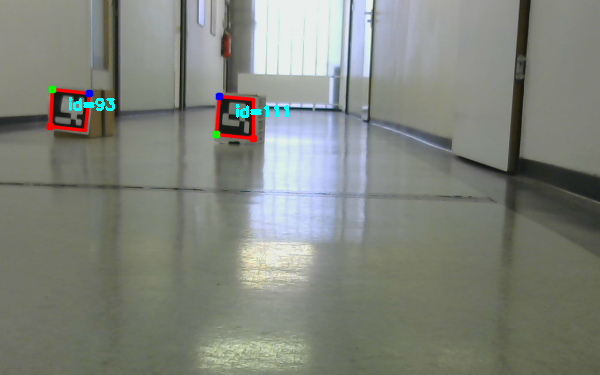
\includegraphics[width=0.9\textwidth]{images/flur.png}
  \caption{\textit{ArUco}-Tor aus Sicht der Kamera}
  \label{fig:ArUco-Tor aus Sicht der Kamera}
\end{figure}
\newline
Dabei können nicht nur die \textit{Id}s der einzelnen Marker ausgelesen werden, sondern auch deren Position im Raum. In der gezeigten Abbildung sehen wir zwei \textit{ArUco}-Marker aus Sicht der Fahrzeugkamera.

	\cleardoublepage
	\section{Projektkoordination}
\label{sec:projektkoordination}

Nicht nur die technischen Voraussetzungen, sondern auch die Organisation im Team stellte einen wichtigen Faktor für den Erfolg dar.

%%%%%%
\subsection{Verantwortungsbereiche}
Zunächst analysierten wir genau sowohl die uns gegebenen technischen Möglichkeiten, als auch die Aufgabenstellung. Daraufhin verteilten wir Verantwortungsbereiche auf die einzelnen Gruppenmitglieder. Einige dieser Bereiche waren:
\begin{itemize}
	\item Code - Verantwortlich für eine lesbare Struktur und Kommentare im Code
	\item Zeitmanagement - Verantwortlich für Zeitplanung und Einhaltung der Fristen
	\item Dokumentation - Verantwortlich für die schriftliche Dokumentation der Team-Absprachen
	\item Vorträge, LateX und einige mehr
\end{itemize}
Es handelte sich dabei ganz bewusst um Verantwortungsbereiche und nicht um Aufgabenteilung. Idee hierbei war, dass die einzelnen Gebiete nicht ausschließlich von dem jeweils Verantwortlichen beachtet oder ausgeführt wurden, sondern die jeweils Zuständigen darauf achteten, dass alle den entsprechenden Rahmen einhielten. So konnte sich jeder auf seine Verantwortlichkeiten konzentrieren, ohne fürchten zu müssen andere Aspekte zu vergessen. Auf diese Weise war eine gegenseitige Kontrolle und Erinnerung an die Einhaltung der Aufgaben gegeben. Jedes Teammitglied konnte sich stets darauf verlassen, dass eine wichtige Information notiert und an alle Fristen und Termine, wie die zweiwöchentlichen Treffen mit dem Betreuer, erinnert wurde.


%%%%%%
\subsection{Zeitplan und Meilensteine}
Um einen Zeitplan erstellen zu können, notierten wir zunächst alle extern vom Veranstalter vorgegebenen Ziele mit der entsprechenden Deadline als Meilensteine in unserem Zeitplan. Dazu zählen unter anderem die Endergebnisse und auch die beiden Vorträge. Nachdem wir uns mit der Technik vertraut gemacht hatten, konnten wir auch zu den Meilensteinen Zwischenziele mit der benötigten Zeit und der daraus folgenden Deadline abschätzen. Daraus ergab sich ein Zeitplan, der die gesamte Bearbeitungszeit über Gültigkeit besaß.
\pagebreak
%%%%%%
\subsection{Dokumentation: \textit{Trello}}
Wie bereits erwähnt, legten wir von Anfang an Wert darauf, Absprachen, Entscheidungen, aber auch offene Fragen immer schriftlich festzuhalten. Dies sollte natürlich möglichst übersichtlich dargestellt, aber auch stets für alle zugänglich sein. Wir entschieden uns für \textbf{Trello}\footnote[1]{https://trello.com/}. Dies ist ein Online-Organisationsboard, zugänglich über eine Website, womit alle Informationen immer aktuell an einem Ort vorlagen. In Trello können einzelne Listen aus Karten erstellt werden um die Themen zu gliedern. Während Listen die Oberthemen repräsentieren, stellen die Karten die Unterpunkte zu den einzelnen Themenbereichen dar.
%%%%%%%%
\begin{figure}[hp] 
  \centering
     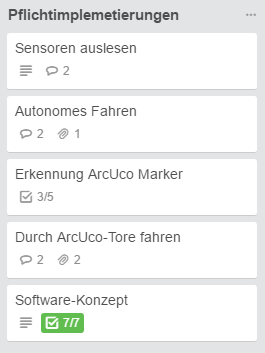
\includegraphics{images/PflichtimplementierungenListe.PNG}
  \caption{Trello-Liste mit Karten}
  \label{fig:Trello-Liste}
\end{figure}
\newline
Dabei werden in der Liste jeweils die Titel der Karten zusammen mit den wichtigsten Informationen angezeigt. So weisen Sprechblasen auf Kommentare und Heftklammern auf Dateianhänge hin. Auch die Anzahl der erledigten Unterpunkte wird angezeigt und bei vollständiger Bearbeitung grün markiert.
\pagebreak \newline
Wählt man nun eine Karte aus, kann man alle weiteren Informationen einsehen. Zuordnungen zu Teilnehmern lassen sich hier realisieren, um, zum Beispiel, Aufgabenteilung oder Verantwortlichkeiten aufzuzeigen. Unterpunkte kann man abhaken, was sich in einem Fortschrittsbalken ablesen lässt. Kommentare mit angehängten Dateien lassen sich ebenso realisieren, wie Verweise auf Karten aus anderen Listen, um Zusammenhänge darzustellen und schnellen Zugriff zu ermöglichen. Am Ende findet sich unter \textit{"`Aktivität"'} ein Log mit allen Ereignissen dieser Karte zusammen mit dem entsprechenden Zeitstempel.

\begin{figure}[hp] 
  \centering
     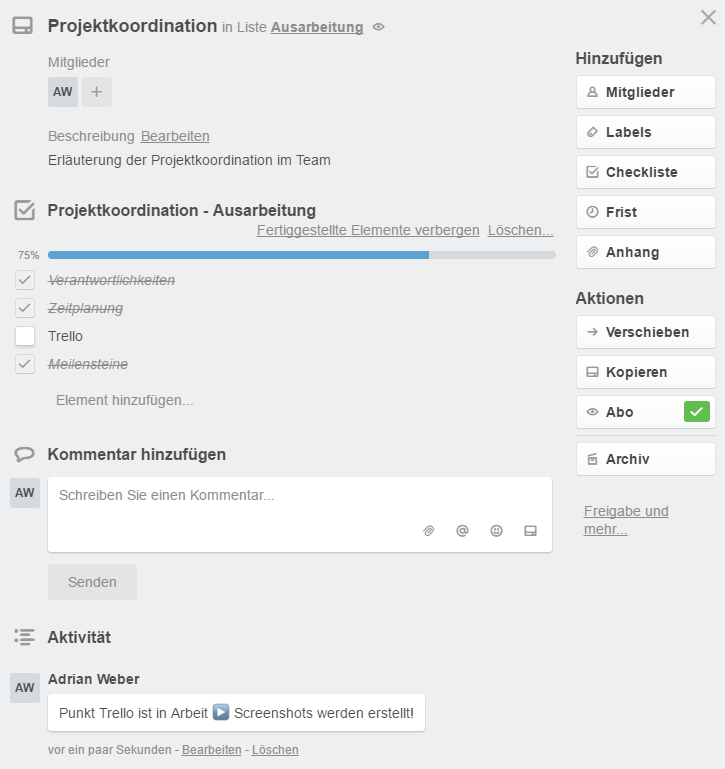
\includegraphics[width=0.9\textwidth]{images/KarteProjektkoordination.PNG}
  \caption{Trello-Karte mit Fortschrittsbalken und weiteren Informationen}
  \label{fig:Trello-Karte mit Fortschrittsbalken, Kommentar und weiteren Informationen}
\end{figure}
	\cleardoublepage
	\section{Aufgabenstellung}
\label{sec:aufgabenstellung}

Im Folgenden soll die genaue Aufgabenstellung, sowie unsere daraus abgeleiteten Themen erläutert werden.

%%%%%%
\subsection{Pflichtimplementierung}
Als Pflichtteil des Projektseminars wurde generell das Thema "`Autonomes Fahren mittels Sensorik"', "`Kamera Inbetriebnahme und Erkennung von ArUco-Markern"', sowie als Anwendung von Letzterem das "`Durchfahren von ArUco-Toren"' vorgegeben.  

Aus dem Standardprogramm abgeleitet haben wir aufgrund der örtlichen Rahmenbedingungen festgelegt, dass sich unser Auto autonom in der vorgegebenen Umgebung bewegen können soll. 
Wir haben folgende Annahmen zur Aufgabenstellung getroffen:
\begin{itemize}
	\item Das Auto hat mindestens eine Wand rechts oder links von sich, zu der es seinen Abstand absolut bestimmen kann
	\item Es wird lediglich mit der vorgegebenen Hardware eine Realisierung des autonomen Fahrens durchgeführt, sodass unser Code auch von nachfolgenden Gruppen einfach genutzt werden kann
	\item Das autonome Fahren wird durch einen Zustandsautomaten realisiert
	\item ArUco-Tore bestehen aus zwei Markern, die in beliebigem Abstand (jedoch begrenzt durch den Kamerablickwinkel) voneinander nebeneinander im Flur stehen
	\item Der Winkel von der Verbindungsgerade zwischen den Markern und den Normalen auf den Markern ist nahe $90^\circ$
	\item Es ist kein starkes Gegenlicht vorhanden, da dies den Kontrast der Kamera stark beeinträchtigt
	\item Die AruCo-Tore befinden sich im gleichen Umfeld, das auch für das autonome Fahren definiert ist
\end{itemize}

%%%%%%
\subsubsection{Vertiefungspakete}
Als optionale Vertiefungspakete wurden "`\textit{ROS}-basierte Simulation"', "`Fernsteuerung und Car-2-Car Kommunikation"', sowie "`Inertialsensorik und erweiterte Regelung"' vorgeschlagen.

Von den vorgeschlagenen Möglichkeiten aufgegriffen:
Regelung: für tordurchfahrt
graphisches Programmierung
Zustandsautomat
XBOX-Kontroller (Hobit)


%%%%%%
\subsubsection{GRUNDLAGE!}
Text
	\cleardoublepage
	\section{L\"osung Pflichtimplementierung}
\label{sec:lsgpflicht}

Wie bereits im Abschnitt "`Aufgabenstellung"' beschrieben, war es Gegenstand der Pflichtimplementierung, dass das Auto autonom mittels Sensorik fahren kann, die Kamera ArUco-Marker erkennt, sowie das Auto durch ein Tor aus solchen hindurchfahren kann. Bereits in obigem Abschnitt wurden die Rahmenbedingungen, welche wir für unsere Lösung angenommen haben definiert. Im Folgenden wird nun erläutert, wie wir, auf Grundlage des Zustandsautomaten, dessen genaue Implementierung erst später erläutert wird, die drei Hauptaufgaben realisiert haben.

%%%%%%
\subsection{Autonomes Fahren}
Unser Konzept zum autonomen Fahren baut sehr stark auf den Möglichkeiten, die uns eine FSM (Finite State Machine/Zustandsautomat) bietet, auf. 
Das Konzept beruht grundlegend darauf, dass das Auto eine FSM lädt, die entweder per JSON-File (genaueres zu JSON, s. Abschnitt 8) oder per graphischer Oberfläche (genaueres zur graphischen Programmierung, s. Abschnitt 9) konfiguriert wird. Die FSM ist ein Graph aus verschiedenen Zuständen, die jeweils eine Funktion des Autos, wie z.B. geradeaus an einer Wand entlang fahren, repräsentieren. Diese verschiedenen Funktionen oder Zustände des Autos sind über Transitionen verbunden, d.h. Ereignisse, die zu einem Zustandswechsel führen. Das kann z.B. eine abrupte Abstandsänderung der führenden Wand sein.
\newline 
Mittels der Kombination aus Zuständen, in denen sich das Auto befinden kann und Ereignissen, die zu einem Zustandswechsel führen, kann ein autonomen Verhalten, je nach Umgebung des Autos realisiert werden. Alternativ kann ein Weg in einem Bekannten Umfeld einprogrammiert werden, indem eine Folge von Zuständen konkateniert wird. 
Der Basiszustand für das autonome Fahren ist ein einfacher Wandfolger-Zustand, der das geregelte Geradeausfahren entlang einer Wand realisiert. 
\newline
\newline
Ein Regelkreis sorgt dafür, dass ein System in einen stabilen Zustand überführt wird. Dazu wird eine Eingangsgröße, in diesem Fall der Abstand zur Wand, in einen Regelkreis geführt. Ausgangsgröße ist dann der Lenkeinschlag, welcher den Abstand des Autos zur Wand beeinflusst. Um nun den Wandabstand stabil zu halten, wird die Differenz zwischen der Regelgröße (Lenkeinschlag) und Führungsgröße (Wandabstand) bestimmt (Regelabweichung). Da die einzelnen Regelkreisglieder ein Zeitverhalten haben, muss der Regler den Wert der Abweichung verstärken, sowie das Zeitverhalten unterdrücken. 
Anfangs haben wir versucht, das Regelverhalten durch einen PID-Regler abzubilden, jedoch führten Tests und Hinweise der Gruppe \textit{Nullpointer} des vergangenen Semesters zu einer Vernachlässigung des I-Anteils. Generell sorgt der P-Anteil für eine proportionale Verstärkung der Regelabweichung. Der D-Anteil sorgt für ein differenzierendes Verhalten, ist also abhängig von der Änderungsgeschwindigkeit der Regelabweichung.
Der vernachlässigte I-Anteil sorgt für eine zeitliche Integration der Regelabweichung. Dies führt bei dem Auto zu einer sich mit höherem I-Anteil einstellenden Trägheit, die das Auto unflexibler macht.

Der Basiscode, mit dem der Regler implementiert wird, ist in der Klasse \textit{BasicFollowWall} (Zeile 53) zu sehen:
\begin{lstlisting}
double y = _p * e + _esum * _i * PID_S + _d * (e - _eold)*PID_INVS;
\end{lstlisting}

Hierbei stellen \textit{PID\_S} und \textit{PID\_INVS} Konstanten dar (0.0125 und 80). \textit{\_p} ist der Proportionalanteil, \textit{\_i} der Integralanteil und \textit{\_d} der Differentialanteil. e ist die Eingangsgröße, \textit{\_esum} die aufaddierten Wandabstände der vergangenen Durchläufe und \textit{\_eold} der Wert des letzten Durchlaufes. \textit{y} ist der daraus berechnete Lenkeinschlag.
\newline
\newline
Mittels des oben vorgestellten PD-Reglers wird im Zustand \textit{BasicFollowWall} das Geradeausfahren implementiert. Erste Tests haben gezeigt, das entgegen der Erwartungen auch Kurven mit dem gleichen Zustand umfahren werden konnten. Daraus ergab sich dann die Einsicht, dass kein neuer Kurvenzustand eingeführt werden musste. Es lassen sich also alle grundlegenden Bewegungen durch eine Konkatenation verschieden parametrisierter Wall-Follow Zustände erreichen. Zudem hat sich herausgestellt, dass Kurven umso besser funktionieren, wenn unmittelbar vorher die Geschwindigkeit gedrosselt wird und im Anschluss ein größerer Wandabstand gewählt wird, da sonst die Gefahr besteht, dass die Ultraschallsensoren einen zu steilen Winkel zur Wand haben. 
Nun ist es also möglich mit einem einzigen Zustand (BasicFollowWall) die grundlegenden Bewegungen (Geradeausfahren, Kurvenfahren) abzudecken. Als Transitionen zwischen den Zuständen haben wir vier Optionen implementiert: \textit{Always, Distance, Finished, SensorLevel}. 
\begin{itemize}
	\item \textbf{Always}: Diese Transition feuert sofort.
	\item \textbf{Distance}: Diese Transition feuert nach der übergebenen Distanz. Die aktuelle Distanz wird immer über die Hall-Sensoren aus dem aktuellen Maschinen-Zustand (Machine State) ausgelesen. 
	\item \textbf{Finished}: Um zu feuern, muss die Methode \textit{isFinished()} des vorangegangenen Zustands \textit{true} zurückgeben. Diese Transition ist also nur möglich, wenn der vorige Zustand das Interface \textit{IFinishable} implementiert. 
	\item \textbf{SensorLevel}:	SensorLevel ist die meistgenutzte Transition. Sie feuert immer dann, wenn ein vorgegebener Sensorwert über oder unterschritten wurde. Diese Transition kann Werte aller drei Ultraschallsensoren als Referenz nehmen und sowohl bei Über- oder Unterschreiten eines Grenzwertes aktiv werden. 
\end{itemize}
Neben dem BasicFollowWall-State sind noch einige weitere States implementiert, die jeweils spezielle Aufgaben erfüllen und im Folgenden knapp vorgestellt werden:
\begin{itemize}
	\item \textbf{ApproachPoint}: Es kann ein Punkt übergeben werden, der dann geregelt angefahren wird. Dieser Zustand wurde von uns dafür erstellt, einen Punkt einen Meter vor einem ArUco-Tor anzufahren.
	\item \textbf{ArucoGateCenter}: Dieser Zustand richtet das Auto aus, wenn es vor einem ArUco-Tor steht, um das Tor anschließend gerade zu durchfahren. Dies ist nötig, da das Auto nach Transition aus dem ApproachPoint-Zustand nicht rechtwinklig zur Verbindungsgeraden der beiden Marker-Mittelpunkte ausgerichtet ist.
	\item \textbf{FollowWall}: FollowWall ist eine Modifikation des BasicFollowWall-Zustandes. Ziel war, dass die Regelung Türrahmen ignoriert, sodass sich das Auto anschließend nicht stark aufschaukelt. Dies wurden erreicht, indem Abweichungen der Ultraschallsensorwerte, die größer als 2cm sind, ignoriert werden. Dies bringt den Vorteil mit sich, dass das Auto sehr stabil gerade aus fährt. Nachteilig ist jedoch, dass es nicht mehr oder nur noch sehr schwach auf größere Änderungen der Umgebung reagiert. Zur Erkennung von Kurven ist dies jedoch kein Problem, da diese ja in der folgenden Transition getriggert werden.
	\item \textbf{FollowWallRamp}: Dieser Zustand ermöglicht eine Abstandsregelung zu einer das Auto umgebenden Wand nach einer linearen Funktion. Er ermöglicht somit z.B. einen Spurwechsel oder das Umfahren von Hindernissen.
	\item \textbf{FSMState}: Dieser Zustand ermöglicht das Einbinden von Zustandsautomaten als eigenen Zustand in einer FSM. Dies schafft eine sehr starke Abstraktion, sodass eine Zustandsfolge, z.B. zur Kurvenfahrt, abstrakt eingebunden werden kann und die Größe des Gesamtautomaten überschaubar bleibt.
	\item \textbf{Idle}: Dieser Zustand macht nichts. 
	\item \textbf{Motor}: Hier fährt das Auto einfach mit festgelegter Geschwindigkeit eine festgelegte Distanz geradeaus.
	\item \textbf{Stop}: Dieser Zustand stoppt das Auto.
\end{itemize}
Mittels der vorgestellten Konstrukte kann nun eine beliebige Abfolge von Aktivitäten des Autos abgebildet werden. Es ist möglich, ihm eine Strecke oder alternativ ein Verhalten einzuprogammieren. Ein autonomes Verhalten wird z.B. über mehrere parallele Zweige im Automaten realisiert. Als Beispiel fährt das Auto geradeaus und falls ein Hindernis auftritt, feuert eine Transition, die mehrere Zustände zu dessen Umfahren triggert. Werden Marker erkannt, könnte eine andere Transition feuern und je nach ID ein Verhalten des Autos auslösen.

Durch die vorgestellte Modularität ist das autonome Verhalten des Autos um (fast) beliebig Szenarien erweiterbar (Fliegen lernen wird es leider ohne Hardwareanpassungen nie können).
%%%%%%
\subsection{Erkennung ArUco-Marker}
Die Erkennung der ArUco-Marker ist durch einen ROS-Node implementiert. Dort haben wir zur Kamerakalibrierung eine Kombination der ROS-internen Kalibrierung und der Kalibrierung der  \textbf{OpenCV}\footnote[1]{http://opencv.org/} Open Source Software Bibliothek verwendet. Zur Kalibrierung wird ein Schachbrettmuster verwendet. Dabei übergibt man der OpenCV-Routine die Anzahl der Kästchen und deren Größe. Nachdem die Eckpunkte erkannt sind, werden verschiedene Orientierungen im Raum dargestellt, um eine robuste Kalibrierung zu erreichen. Anhand der Zuordnungen von Raum zu Bildkoordinaten kann nun die Kalibrierungsmatrix berechnet werden. 
OpenCV erkennt nun die ArUco-Marker und kann deren Position errechnen. Die Daten dazu werden anschließend in einer ROS-Topic gepublisht. Unserer Anwendungssoftware stehen so die genauen Bildkoordinaten der Marker und ihre Ausrichtung im Raum zur Verfügung.  

%%%%%%
\subsection{Durchfahren von Toren}
Nachdem nun dargestellt wurde, wie ArUco-Marker erkannt werden, bedarf es nur noch eines weiteren Schrittes, um das erkannte ArUco-Tor zu durchfahren. Man muss anhand der erhaltenen Koordinaten den weiteren Streckenverlauf so umplanen, dass das Tor durchfahren wird. 
\newline
Dazu gibt es verschiedene mögliche Ansätze. Zuerst war geplant, eine S-Kurve zu berechnen, deren Startpunkt die aktuelle Position und deren Endpunkt ein Punkt unmittelbar vor dem ArUco-Tor ist. Der Vorteil dieser Implementierung ist, dass das Auto vor dem Tor schon senkrecht zur Verbindungsstrecke der beiden Markermittelpunkte ausgerichtet ist, sodass es dann nur noch geradeaus fahren muss. Dazu war es nötig, sowohl Kenntnis über die Strecke, welche durch eine Hallsensoreinheit beschrieben wird, sowie über die Lenkwinkel, passend zu den eingestellten Lenkeinschlägen, zu erhalten. Dazu haben wir mehrere Messstrecken durchgeführt. Leider lieferte der Hall Sensor teils unzuverlässige Werte. Für die Bestimmung der Lenkwinkel haben wir eine ganze Messreihe aufgenommen. Daraus konnten nun zwei Viertelkreisbögen errechnet werden, die umgekehrt zusammengesetzt eine S-Kurve ergeben. Dabei haben wir festgestellt, dass das Auto bei Lenkeinschlag 0 nicht exakt geradeaus fährt, weshalb ein Offset abgezogen werden musste. Zudem erzielten wir nicht reproduzierbare Ergebnisse. Manchmal fuhr das Auto perfekt durch das erkannte Tor, manchmal lag es weit daneben. Dieser Umstand ist nach unseren Auswertungen dem schlechten Gewichts-Leistungsverhältnis geschuldet. Die Servomotoren schaffen es nicht, gerade aus dem Stand, in den gewünschten Lenkeinschlag zu lenken. Dies führt dazu, dass das Ergebnis von zwei Eingangsgrößen, dem aktuellen Lenkeinschlag und der Geschwindigkeit, abhängt, sodass es uns nicht möglich war diesen Ansatz weiter zu verfolgen. 
\newline
\newline
Daher haben wir uns entschlossen, wie oben bereits erwähnt, eine lineare Regelung zu implementieren. Dies bedingt jedoch (im Gegenteil zur Lösung mittels S-Kurve) eine Wand auf einer Seite des Fahrzeuges, zu der es sich relativ bewegen kann. 
\newline
\newline
Der Regler um eine lineare Funktion erhält als Eingangsgrößen den Startabstand, den Endabstand, sowie die Strecke in Hallsensoreinheiten. Anhand dieser Werte wird, wie auch im normalen \textit{BasicFollowWall}-State, eine Regelung durchgeführt. Unterschied ist diesmal jedoch, dass sich der Abstand zur Wand, der sonst ja konstant ist, linear ändert. Das heißt, dass die Regelung mit zunehmender zurückgelegter Strecke, was durch den Hallsensor ermittelt wird, um einen weiter von der Wand entfernten Abstand regelt. 
\newline
\newline
Diese Funktion wurde im \textit{FollowWallRamp}-State implementiert. In diesem State gibt es eine Funktion, \textit{setTarget(Vec3f target)}, die den Zielpunkt der Regelung festlegt. Dazu wird, je nach Wandseite, die x-Koordinate den übergebenen Werten angepasst. Dabei wird die x-Koordinate des Ziels um den aktuellen Wandabstand erhöht bzw. erniedrigt, sodass sie den wirklichen Wandabstand enthält. Des Weiteren wird der y-Abstand des Zielpunktes für die messbaren Halldistanzwerte normalisiert.
\newpage
\begin{lstlisting}
void FollowWallRamp::setTarget(Vec3f target)
{
_finished = false;
if(_wallSide == WallSide::Right)
_targetClearance = -(target[0])+_startClearance;
else
_targetClearance = target[0]+_startClearance;
_distance = 1500/1.60f*target[2];
}
\end{lstlisting}

In der \textit{tick()}-Methode sind nur folgende fünf Befehle relevant:

\begin{lstlisting}
unsigned int curDistance = mstate.getHallDistance()-_startDistance;

if(curDistance >= _distance)
_finished = true;

double m = (_targetClearance-_startClearance)/(_distance);
_clearance = m*curDistance + _startClearance;
...
BasicFollowWall::tick();
\end{lstlisting}

Hier wird die aktuell zurückgelegte Distanz aktualisiert und mit der Zieldistanz verglichen. Sollte diese erreicht sein, wird die nächste Transition gefeuert, indem der Wert \textit{\_finished}, der aufgrund der Implementierung des \textit{IFinishable}-Interfaces vorhanden sein muss, gesetzt wird. Ansonsten wird die aktuelle Steigung berechnet, sowie mit ihr der aktuelle Wandabstand \textit{\_clearance}. Mit diesem wird am Ende der \textit{tick()}-Methode des \textit{FollowWallRamp}-Zustands die \textit{tick()}-Methode des \textit{BasicFollowWall}-Zustands aufgerufen. Dies sorgt wie im Standardfall auch für eine Regelung um den festgelegten Wandabstand. 
\newline
Wie man sehen kann, ist für die Regelung nach einer linearen Funktion nur eine geringe Änderung des vorhandenen Codes nötig gewesen. 
\newline

\begin{figure}[htbp] 
	\centering
	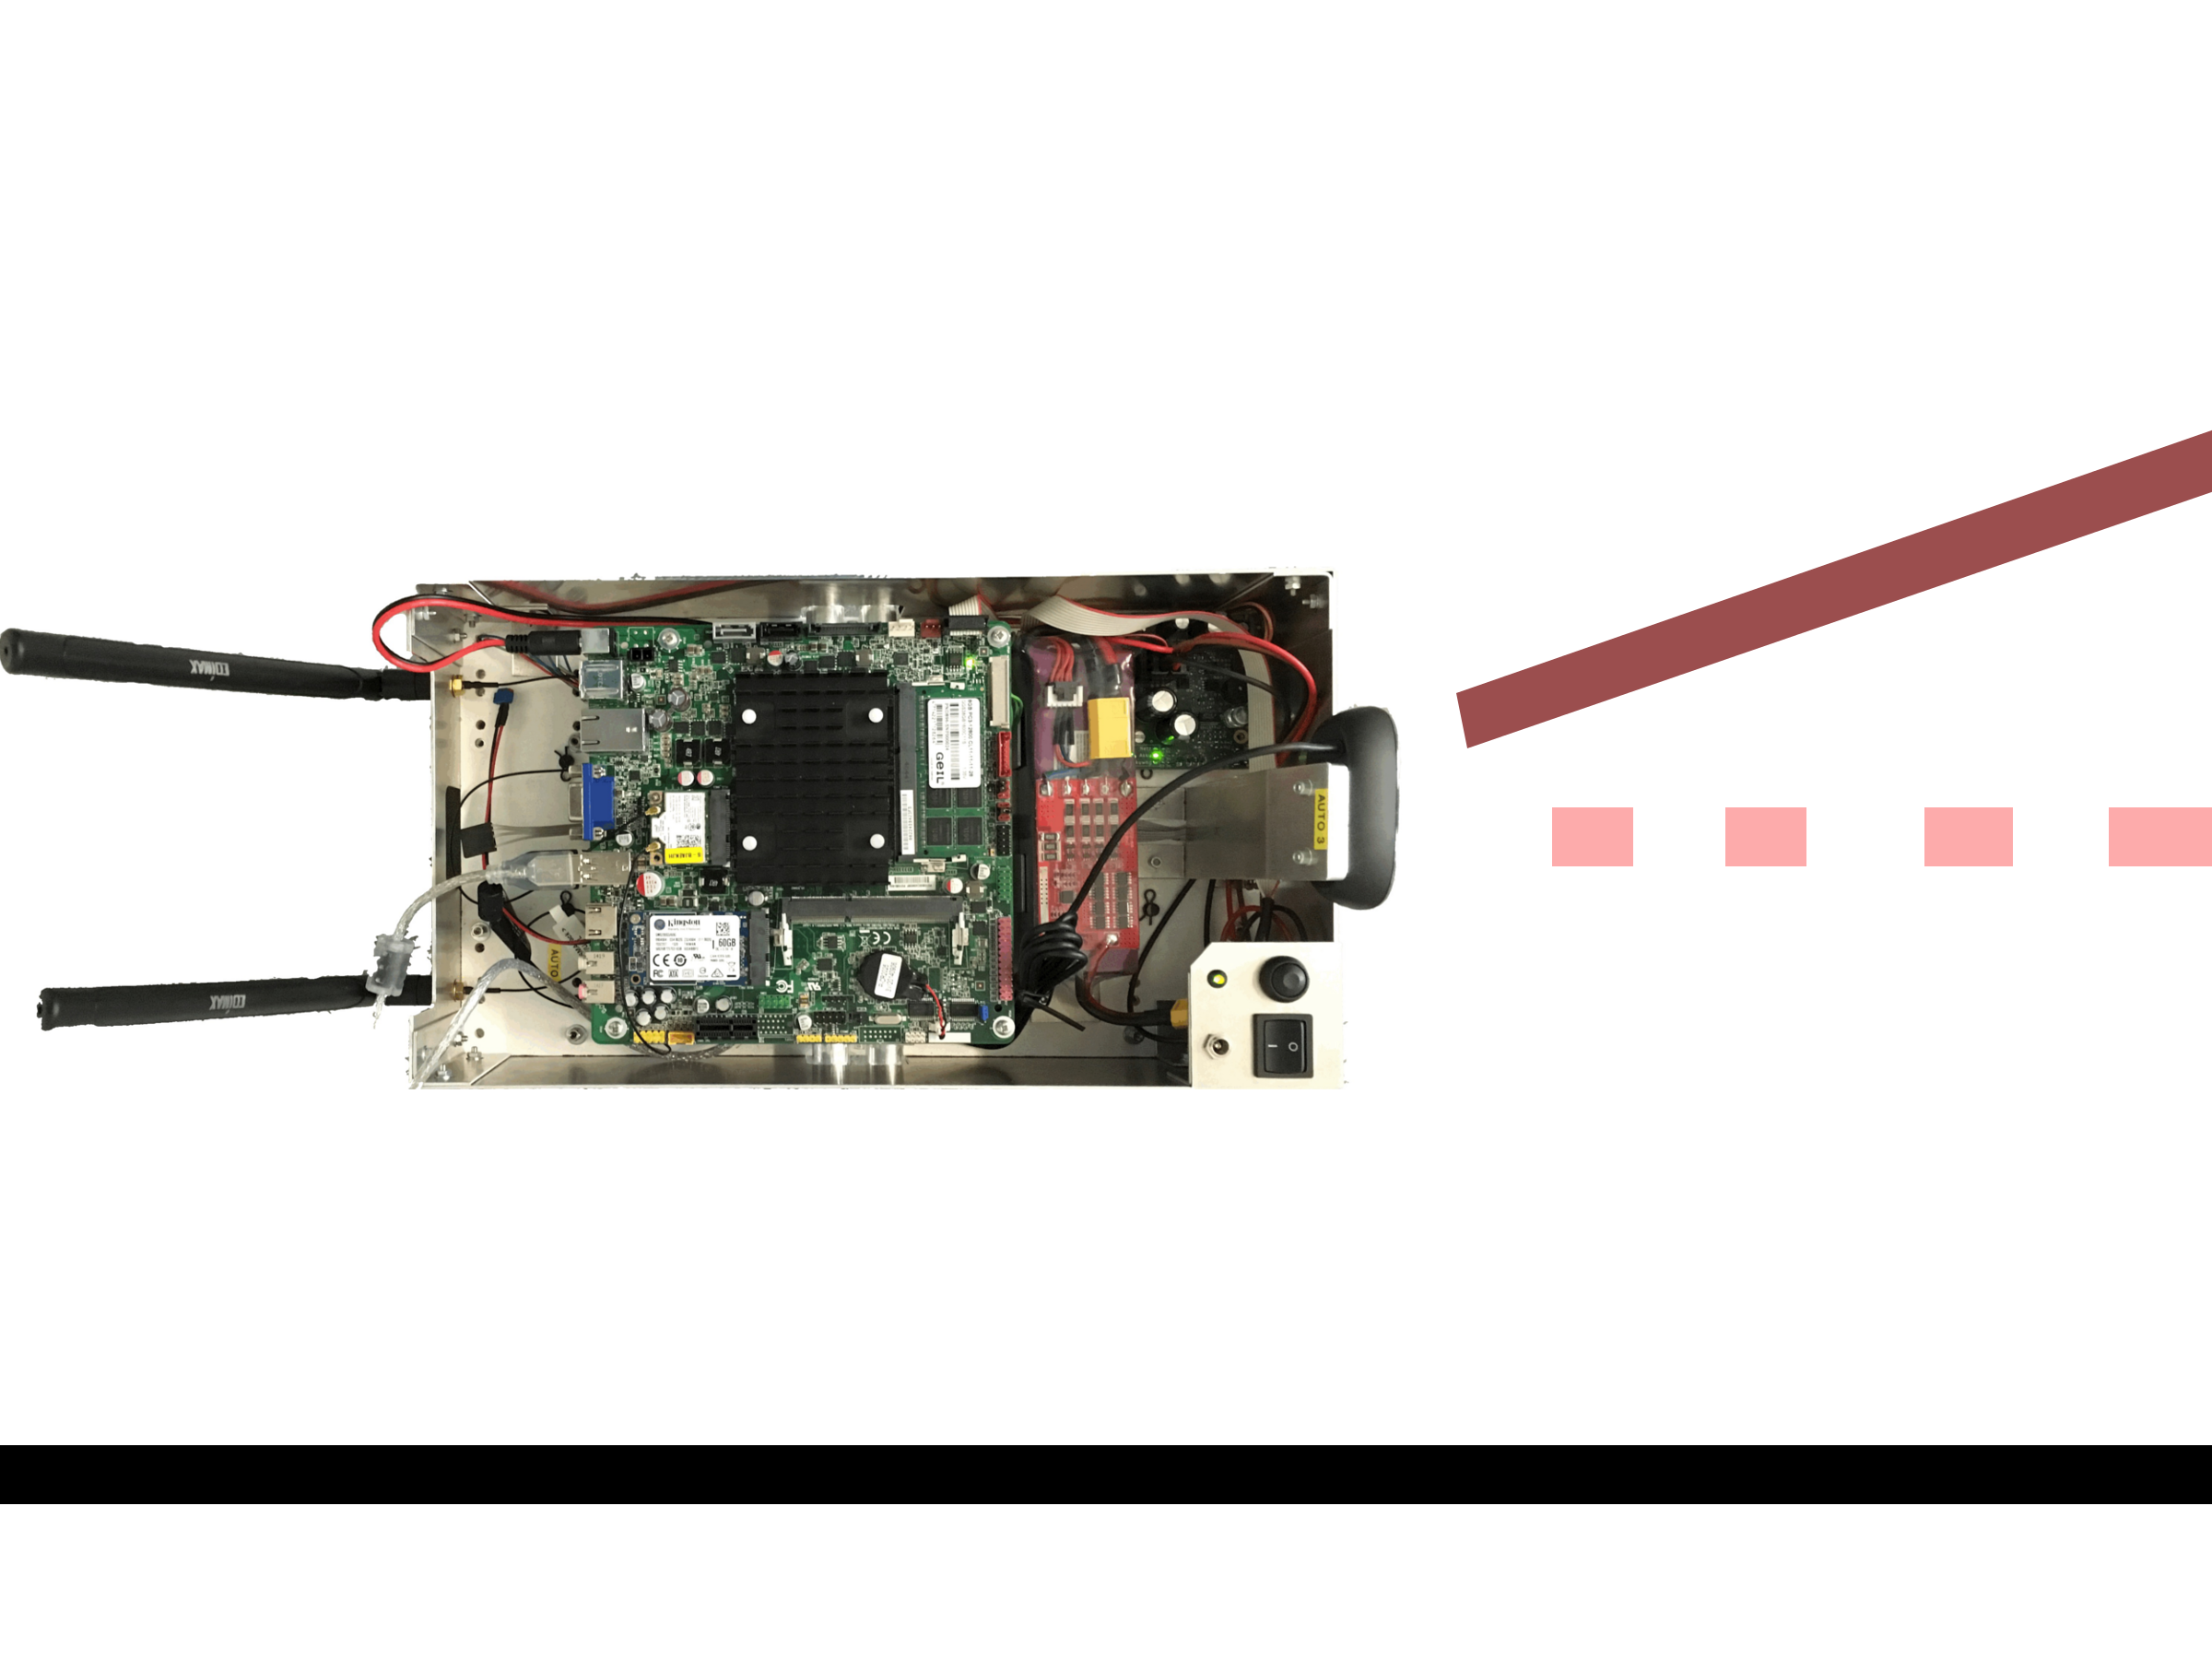
\includegraphics[width=250pt]{images/scharfeRampe.png}
	\caption{Schematische Darstellung des Fahrens einer Rampe}
	\label{fig:ScharfeRampe}
\end{figure}

Diese neue Funktion des Autos wurde nun von uns verwendet, um ein durch die Kamera erkanntes ArUco-Tor, dessen Koordinaten im Raum übergeben wurden, auf einen Punkt einen Meter vor dem Tor anzusteuern.
Weiter oben wurde bereits der Umstand erwähnt, dass es mit einer S-Kurve möglich ist, eine gerade Ausrichtung des Autos zu erreichen. Dies ist mit der Rampenfunktion nicht möglich. Vielmehr ist die Ausrichtung fast nie gleich, da durch die Regelung unterschiedliche Lenkwinkel angenommen werden. In der Regel ist das Auto jedoch in Fahrtrichtung um einen geringen Winkel zwischen $0^\circ$ und $45^\circ$ zur Parallelen zur Wand durch den Tormittelpunkt versetzt. Daher muss die gefeuerte Transition nun noch in zwei weitere Zustände, einen zum Ausrichten des Autos (ArucoGateCenter) und einen zum geradeaus fahren (Motor), überführen. Ersterer macht nichts anderes, als zu prüfen, ob der Tormittelpunkt auf der linken oder rechten Seite des Autos ist und den Lenkeinschlank in entsprechender Richtung auf 1.0 zu setzen und das Auto so weit zu bewegen, bis es ausgerichtet ist. Der Motor-State liest aus seiner JSON-Konfiguration den übergebenen Lenkeinschlag und die Geschwindigkeit und fährt mit dieser Konfiguration so lange, bis die folgende Transition feuert. 
\newline
\newline
Wie man sehen kann, benötigen wir lediglich drei Zustände, um die Tordurchfahrt zu realisieren. Dank unserer FSM-Struktur ist es uns so einfach möglich, z.B. indem das Erkennen und Durchfahren eines ArUco-Tores parallel zu einem anderen Pfad geschaltet wird, flexibel auf auftauchende Tore zu reagieren und diese zu durchfahren. 
  
	\cleardoublepage
	\section{FSM}
\label{sec:fsm}
Wir betrachten nun etwas genauer wir unsere Konzept einer FSM zur 
Kontrollflusssteurung in C++11 umgesetzt haben, dazu gehört neben der Wahl 
der Klassenstruktur auch die Einbindung nützlicher Features von C++11 um die
Speicherverwaltung zu optimieren.


%%%%%%
\subsection{Klassenstruktur}
Zur Modellierung einer FSM haben wir ein Konzept aus einer Kontroller Klasse \texttt{FSM} und zwei abstrakten Basisklassen \texttt{State} und \texttt{Transition} überlegt. Dabei stellen die abstrakten Basisklassen nur eine standardisiertes Interface bereit und erlauben somit einen schnelle Implementation von neuen abgeleiteten Klassen.


Erst die abgeleiteten Klassen implementieren eine genau Funktionalität, wie z.B. einer Wandfolgen oder eine Transition nach einem bestimmten Ereignis. Diese Klassen sind in dem dafür vorgesehen namespace \texttt{TRAL::STATES} und \texttt{TRAL::TRANSITIONS} zu finden.

\begin{figure}[htbp] 
  \centering
     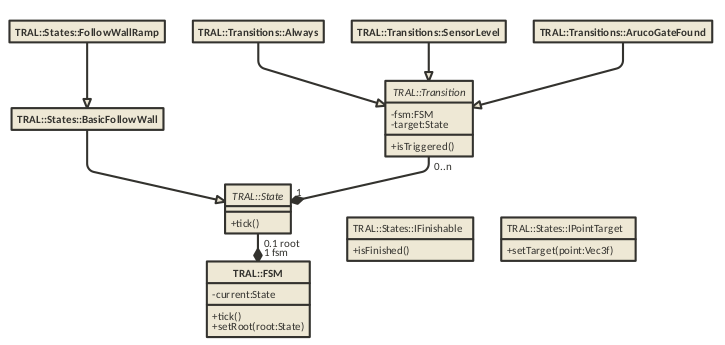
\includegraphics[width=\textwidth]{images/fsm-uml.png}
  \caption{Vereinfachtes Klassendiagram der FSM}
  \label{fig:KlassendiagramFSM}
\end{figure}

%%%%%%
\subsubsection{FSM}
Die Klasse \texttt{FSM} implementiert die komplette Kontrollflusssteuerung und kümmert sich ebenso um das Laden einer FSM die zuvor graphisch mit Umlet erstellt wurde. Ebenso hält diese Klasse immer eine aktuelle Referenz zum dem globalen \texttt{MachineState}, in dieser Klasse sind alle Sensorinformationen aufbereitet konsolidiert.

\paragraph{\texttt{FSM::tick}}

Die wichtigste Funktion diese Klasse ist die \texttt{tick} Funktion, diese wird zyklisch von der Rosnode tral-fsm aufgerufen. Dabei wird der Kontrollfluss an den aktuell aktiven State weitergeben. Wenn nun der aktive State einen neuen Ausgabe gesetzt hat und die Kontrolle wieder abgibt werden nun alle an diesen State befindlichen Transition überprüft ob diese Ausgelöst haben, sollte dies der Fall sein wird eine \texttt{transit} vollzogen.

\paragraph{\texttt{FSM::transit}}

Beim Statewechsel wird zuerst dem aktuell noch aktiven State signalisiert das der nun verlassen wird, dabei kann der State
zum Beispiel genutzte Ressourcen wieder freigeben. Darauf folgend wird dem neuen State signalisiert das dieser nun betreten wird und nötige Ressourcen belegen kann.


%%%%%%
\subsubsection{State}
Die Klasse \texttt{TRAL::State} ist eine abstrakte Basisklasse von dieser werden alle States abgeleitet, für unsere implementation wurden zum Beispiel folgende States abgeleitet:

\begin{itemize}
	\item ApproachPoint
	\item ArucoGateCenter
	\item BasisFollowWall
	\begin{itemize}
		\item FollowWall
		\item FollowWallRamp
	\end{itemize}
	\item Idle
	\item Motor
	\item Stop
\end{itemize}

Jeder instantiierbarer State muss alle virtuellen Funktion der State Klasse implementieren. Dadurch wird gewährleistet das die FSM Klasse mit jede beliegen State Implementation arbeiten kann.

Die statische Funktion \texttt{createFromJson} erlaubt ein State Instanz aus einem JSON Objekt erzeugen Als virtuelles Interface sind die Funktion \texttt{tick}, \texttt{onEnter}, \texttt{OnExit} und weitere Debug-Funktionen vorgesehen.

\texttt{onEnter} und \texttt{OnExit} signalisieren das zuvor beschriebene betreten und verlassen eines States bei der Ausführung. Die Funktion \texttt{tick} wird für den aktiven State zyklisch ausgeführt und berechnet einen neue Ausgabe. Dabei kann über den globalen \texttt{MachineState} auf die aktuellen Sensorwerte zugegriffen und die Aktoren angesteuert.


%%%%%%
\subsubsection{Transition}
Ähnlich der State Klasse fungiert die \texttt{TRAL::Transition} als abstrakte Basisklasse für alle Transitionen. Ebenso existiert auch eine statische Funktion \texttt{createFromJson} um gespeicherte Instanz aus einem JSON Objekt zu laden. 

Jede Transition gehört zu einen eindeutigen Besitzer \textit{owner} und zu einem eindeutigen Ziel \textit{target}. Sollte der \textit{owner} State aktuell aktiv sein wird jene Transition auf Auslösung, mit der Funktion \texttt{isTriggerd}, durch die FSM Instanz nach der Ausführung des States überprüft.

Für unsere Implementierung haben wir folge Transitionen abgeleitet:

\begin{itemize}
	\item Always
	\item ArucoGateFound
	\item Distance
	\item Finished
	\item SensorLevel
\end{itemize}

%%%%%%
\subsubsection{Interfaces}

Um die Übergabe von Informationen zwischen zum Beispiel einem State und einer Transtion zu gewährleisten haben wir zwei Interfaces für States verwendet. 
States die das Interface \texttt{IFinishable} einbinden können entscheiden wenn diese Abgeschlossen sind. Zum Beispiel implementiert der State \texttt{ApproachPoint} diese Interface und signalisiert die Ankunft an dem definierten Punkt.

Ebenso können States die das Interface \texttt{ApproachPoint} implementieren ein Zielpunkt gesetzt bekommen. Diese Interface wird auch zum Beispiel vom State \texttt{ApproachPoint} implementiert und erlaubt so ein verlegen des definierten Punktes bei der Ausführung.

Soll muss zum Beispiel der \textit{owner} State der \texttt{Finished} Transition das dazugehörige Interface implementieren, sollte dies nicht der Fall sein kommt es zu einem Laufzeitfehler während der Ausführung.

	\cleardoublepage
	\newcommand\JSONnumbervaluestyle{\color{blue}}
\newcommand\JSONstringvaluestyle{\color{red}}

% switch used as state variable
\newif\ifcolonfoundonthisline

\makeatletter

\lstdefinestyle{json}
{
  showstringspaces    = false,
  keywords            = {false,true},
  alsoletter          = 0123456789.,
  morestring          = [s]{"}{"},
  stringstyle         = \ifcolonfoundonthisline\JSONstringvaluestyle\fi,
  MoreSelectCharTable =%
    \lst@DefSaveDef{`:}\colon@json{\processColon@json},
  basicstyle          = \ttfamily,
  keywordstyle        = \ttfamily\bfseries,
}

% flip the switch if a colon is found in Pmode
\newcommand\processColon@json{%
  \colon@json%
  \ifnum\lst@mode=\lst@Pmode%
    \global\colonfoundonthislinetrue%
  \fi
}

\lst@AddToHook{Output}{%
  \ifcolonfoundonthisline%
    \ifnum\lst@mode=\lst@Pmode%
      \def\lst@thestyle{\JSONnumbervaluestyle}%
    \fi
  \fi
  %override by keyword style if a keyword is detected!
  \lsthk@DetectKeywords% 
}

% reset the switch at the end of line
\lst@AddToHook{EOL}%
  {\global\colonfoundonthislinefalse}

\makeatother

\section{JSON}
\label{sec:json}
Da bei unserer Lösung die Logik zur Steuerung des Autos, also der Zustandsautomat, von der konkreten Implementierung getrennt wird, benötigten wir eine Möglichkeit diesen Automaten zu erstellen, zu speichern und einzulesen.
Unsere Wahl fiel auf die „JavaScript Object Notation“ (JSON), einem einfachen und kompakten Datenformat, welches alle benötigten Funktionalitäten mitbringt und für das es bereits einige Parser für verschiedene Programmiersprachen gibt. Hauptsächlich war unsere Wahl allerdings durch die einfache Lesbarkeit des Codes begründet, da wir zu Beginn des Projektes die Automaten per Hand eintippten.
Eine JSON-Datei besteht im Wesentlichen aus Objekten, welche in geschweiften Klammern gekapselt sind. Diese Objekte bestehen aus beliebig vielen Eigenschaften, die einen eindeutigen Schlüssel und einen zugeordneten Wert haben. Arrays von Objekten sind in eckigen Klammern eingeschlossen. Eine vereinfachte Ansicht eines Automaten könnte also so aussehen:

\begin{figure}[thp]
\begin{tabular}{c}
\begin{lstlisting}[style=json]

{"root": 0,
 "states":
    [{"id": 0,
     "type": "WandFolgen",
     "p": 12,
     "i": 0,
     "d": 30},       
    {"id": 1,
     "type": "FollowWall",
     "p": 12,
     "i": 0,
     "d": 30}],
 "transitions": [ ... ]
}

\end{lstlisting}
\end{tabular}
\centering
\caption{Bla}
\end{figure}
Um diese JSON-Datei zu deserialisieren, also konkrete Objekte unserer Zustände und Transitionen zu erstellen, benötigten wir einen Parser der dazu in der Lage ist. Wir verwenden hierzu die JSON-Library „JSON for modern C++“ von Niels Lohmann(Quelle).
Die komplette Implementierung dieser Library befindet sich in einer einzigen Datei, der „json.hpp“, die in unserer „FSM.cpp“ inkludiert wird.
Für unsere Zwecke verwenden wir den Iterator der Library um mittels for-Schleife über alle Zustände und Transitionen iterieren zu können und die „parse“-Funktion um aus gegebenen Strings ein JSON-Objekt erstellen zu können.
Der genaue Vorgang des Einlesens wird im nächsten Abschnitt erläutert.
	\cleardoublepage
	\section{Graphische Programmierung}
\label{sec:graphischeprogrammierung}

Trotz der einfachen Lesbarkeit der JSON-Datei, verliert man bei immer größer
werdenden Automaten leicht den Überblick und der Vorteil der Trennung von Logik
und Programmierung geht verloren. Um dieses Problem zu beheben setzen wir das
Programm „\textbf{UMLet}“ \footnote[1]{http://www.umlet.com} ein. Es ist ein freies Open-Source UML-Tool, welches mehrere
Diagramm-Arten unterstützt, unter anderem State-Charts. Gespeichert werden
diese Diagramme im xml-Format, welches wir mit dem Programm „\textbf{xml2json}“ \footnote[2]{https://github.com/Cheedoong/xml2json}
in eine JSON-Datei, für die weitere Verwendung, umwandeln.
%%%%%%
\subsection{UMLet - Das Programm}
\begin{figure}[ht]
\centering 
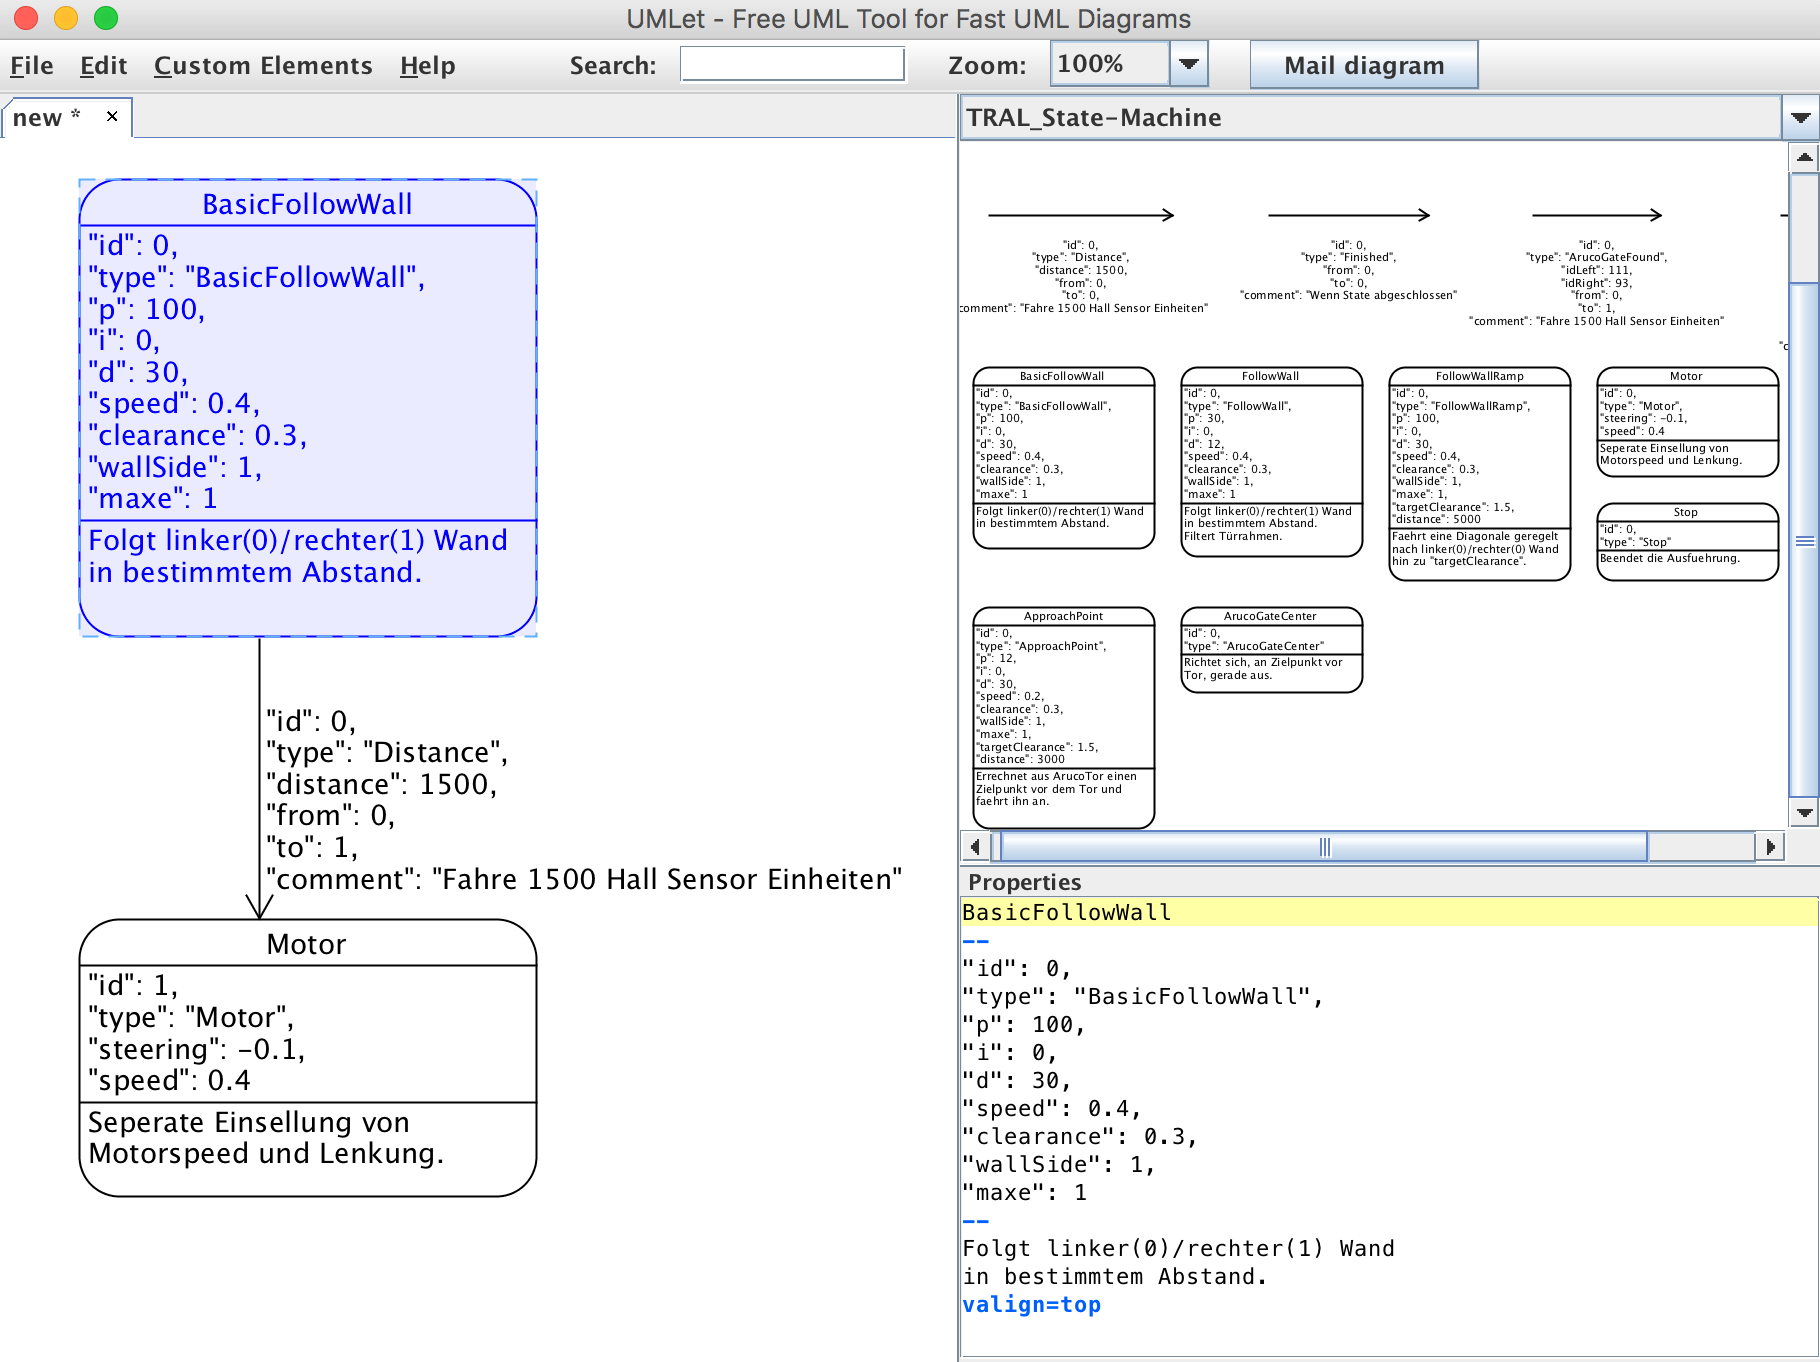
\includegraphics[width=0.90\textwidth]{images/umlet-bsp.png} 
\caption{UMLet Oberfläche}
\label{fig:umlet}
\end{figure}

Das Programm UMLet besteht aus drei Teilbereichen. Im linken Teil, dem
Arbeitsbereich, wird der eigentliche Automat erstellt. Hierfür können schon
vordefinierte Zustände und Transitionen aus der Vorlage „TRAL\_State-Machine“,
oben rechts im Fenster, in den Arbeitsbereich gezogen und entsprechend den eigenen Wünschen
miteinander verbunden werden. Die Vorlagen-Datei „TRAL\_State-Machine.uxf“ muss
hierfür innerhalb des Programmordners unter „\textit{../palettes}“ hinterlegt sein.
Sie kann natürlich ebenfalls von dort geöffnet und gegebenenfalls erweitert
werden.
Der wichtigste Bereich ist das Fenster für die Eigenschaften der Objekte unten rechts in der Ecke.
Bei Zuständen werden zwischen den beiden horizontalen Trennlinien, bei
Transitionen direkt unter dem stilisierten Pfeil \textit{lt=->}, alle Parameter
angegeben, die zur späteren Erstellungen der Objekte benötigt werden. Diese
Liste muss stets vollständig sein. Sie ist durch unsere konkrete
Implementierung im Quellcode vorgegeben.
Wichtig hierbei ist, den Zuständen und Transitionen eindeutige „\textit{ids}“ zu
vergeben, da diese grundlegend für den logischen Fluss sind.


%%%%%%
\subsection{uxf-Datei in JSON-Format umwandeln}
Die uxf-Dateien, welche von UMLet erstellt werden, sind intern im xml-Format
gespeichert. Sofern man das Tool "xml2json" bereits heruntergeladen und
kompiliert hat, lassen sich diese Dateien mittels des einfachen Konsolen-Befehls

\begin{figure}[thp]
\begin{lstlisting}[style=json]
./xml2json automat.uxf >> automat.json

\end{lstlisting}
\centering
%\caption{Aufbau einer einfachen JSON-Datei}
\end{figure}

in eine JSON-Datei umwandeln.
Da man mittels des Aufrufs „xyz“ unseren FSM-Node starten kann und ihm diese
JSON-Datei übergeben muss, lässt sich dieser ganze Abschnitt leicht mit einem
Shell-Skript zum Umwandeln und Starten der FSM realisieren.


%%%%%%
\subsection{Einlesen einer JSON-Datei}
Unsere Klasse „\textbf{FSM}“ besitzt eine Methode namens „\textit{loadFile}“, welche den Automaten
im JSON-Format einlesen kann. Die Implementierung muss natürlich an den Aufbau
der Datei durch das graphische Tool angepasst sein. Die resultierende
JSON-Datei besteht aus zwei geschachtelten Objekten mit verschieden Angaben zum
Programm und zur Programmversion. Im inneren Objekt ist eine Eigenschaft mit dem
Schlüssel „\textit{element}“ angelegt. Diese Eigenschaft enthält ein Array aller Zustände
und Transitionen.
Mittels der Anweisung \texttt{j["diagram"]["{}element"]} greift man
darauf zu und kann mittels des Iterators \texttt{auto jelem} darüber iterieren.

\begin{figure}[thp]
\begin{lstlisting}[style=json]
for(auto jelem: j["diagram"]["element"])

\end{lstlisting}
\centering
\caption{FSM.cpp, Zeile 32}
\end{figure}

Jedes Element besteht aus vier Eigenschaften: \textit{id}, \textit{coordinates},
\textit{panel\_attributes} und \textit{additional\_attributes}. Relevant ist die \textit{id}, um
zwischen Zuständen und Transition zu unterscheiden und die „panel\_attributes“.
Hier ist ein String mit der Parameterliste gespeichert.

Es muss insgesamt zwei Mal über alle Elemente iteriert werden. Beim ersten
Durchgang werden alle Zustände erstellt, beim Zweiten alle Transitionen. Dies
ist deshalb notwendig, weil alle Transitionen einen Verweis auf ihren Vor- und
Nachfolgezustand enthalten. Um diesen Verweis erstellen zu können, muss das
entsprechende Zustandsobjekt bereits existieren.

Der String der Parameterliste enthält noch Steuerzeichen und es wird, je
nachdem, ob Zustände oder Transitionen erstellt werden, die Funktion
\texttt{manipulateString} entsprechend aufgerufen, um diese zu entfernen. Der
verbleibende String ist jetzt ebenfalls nach dem Schema eines JSON Objektes
aufgebaut und enthält Eigenschaften mit Schlüsselwort und zugeordnetem Wert.
Daraus kann nun ein JSON-Objekt erstellt werden:

\begin{figure}[thp]
\begin{lstlisting}[style=json]
json jstate = json::parse(jstr);

\end{lstlisting}

\centering
\caption{JSON-Objekt erstellen, FSM.cpp, Z.37}
\end{figure}


Für ein solches JSON-Objekt hatten wir bereits in den Zustands- und
Transitionsklassen Methoden implementiert, die daraus konkrete Objekte für unsere
FSM erstellen können (\textbf{Transition.cpp} / \textbf{State.cpp}).
Hier kann, an Hand der Information die unter dem Schlüssel \texttt{type} im JSON-Objekt
gespeichert ist, entschieden werden, welche Art von Zustand/Transition vorliegt
und der entsprechende Konstruktor aufgerufen werden.
Im Falle eines Zustandes ist das Prozedere des Einlesens beendet und das
Zustandsobjekt wird in einem Array am Index seiner \textit{id} gespeichert.

\begin{figure}[thp]
\begin{lstlisting}[style=json]
states[(int)jstate["id"]] = state;

\end{lstlisting}
\centering
\caption{Array mit Zuständen, FSM.cpp, Z.39}
\end{figure}



Bevor Transitionen in ihrem Array gespeichert werden können, müssen zuvor noch
Vorgänger und Nachfolgezustand gesetzt werden. Ebenso wird dem Vorgängerzustand
die von ihm abgehende Transition zugeordnet.

\begin{figure}[thp]
\begin{lstlisting}[style=json]
trans->setOwner(states[from]);
trans->setTarget(states[to]);
states[from]->addTransition(trans);

\end{lstlisting}
\centering
\caption{Behandlung von Transitionen, FSM.cpp, Z.53-56}
\end{figure}


	\cleardoublepage
	\section{Doku}
\label{sec:doku}

Hallo?

%%%%%%
\subsection{Noch grundlegender}
Text

%%%%%%
\subsubsection{Grundlage?}
Test

%%%%%%
\subsubsection{GRUNDLAGE!}
Text
	\cleardoublepage
	\section{Fazit}
\label{sec:fazit}
\subsection{Das Fahrzeug}
Die durch das Projektseminar Echtzeitsysteme gewonnenen Erfahrungen sind sehr vielschichtig. Wie schon in der Einleitung zu vermuten war, galt es technisch gesehen Hürden aus den unterschiedlichsten Bereichen zu überwinden. Von Verständnis von komplexer Software wie \textit{ROS} und Einsicht in das eingesetzte Linux Echtzeitbetriebssystem zu erlangen, bis zur Änderung der Software auf dem \textit{Fujitsu}-Board. Auf der anderen Seite vom Interpretieren und Verwenden der Sensorwerte bis hin zum Ansteuern der Motoren und ermitteln der Regler-Werte. Im Laufe der Bearbeitungszeit stellten wir schnell fest, dass vor allem in der Hardware die Schwierigkeiten lagen. Dabei war weniger die Prozessorleistung oder Rechengeschwindigkeit das Problem, diese reichte auch für das Verarbeiten des Videostroms, als vielmehr die Sensorik, Aktorik und der Aufbau des Fahrzeugs. Selbst mit eigens entwickelter Filterung waren die Ultraschall Werte nicht immer zuverlässig, vor allem, wenn der Winkel zum reflektierenden Objekt ungünstig war, als ganz besonders an Ecken und Kanten. Da diese in den Fluren des Instituts jedoch oft ähnlich aufgebaut waren, ließ sich auch hier mit Software ganz gut Abhilfe schaffen. Deutlich problematischer erwies sich der Hall-Sensor. An der Grenze der Erreichbarkeit *bessere Formulierung?* angebracht, reichte es schon beispielsweise beim Einschalten den Aufbau gegenüber dem Fahrgestell zu verschieben. Somit wurde der Abstand gegenüber der im Rad montierten Magnete minimal vergrößert und eine Messung unmöglich. Auch entdeckten wir nicht immer erklärbare Sprünge *kann man das so sagen?* der Hall-Sensor-Werte, was verständlicherweise ein präzises Fahren sehr erschwerte. Als recht umständlich erwies sich auch die Lenkung. Nicht der große Wendekreis und das langsame Einlenken, unter anderem verursacht durch den schweren Aufbau, stellten hier die größte Schwierigkeit dar. Sondern vor allem die Nichtlinearität, die zudem in jede Richtung unterschiedlich war. Einen Pfad zu berechnen und das Fahrzeug entsprechend zu steuern stellte sich, wie in Kapitel 7.3 bereits beschrieben, als stellenweise sehr unpräzise heraus. Wir haben daher wieder auf eine Regelung, unterstützt von einer geraden Wand zurückgegriffen, was für unsere Zwecke sehr gut funktionierte, das allgemeine Problem mit der Lenkung jedoch nur umgeht. Die Kamera funktionierte nach korrektem Kalibrieren und Ansprechen mit \textit{ROS} recht zuverlässig. Hier haben wir lediglich den Aufbau etwas modifiziert und den Neigungswinkel der Kamera leicht aufgerichtet, sodass wir vor dem Fahrzeug mehr Strecke überwachen konnten.

%%%%%%%%%%
\subsection{Projektkoordination und Aufgabenstellung}
Die Projektkoordination war ebenfalls ein wichtiger Aspekt, den wir bedenken mussten. Unser Vorgehen basierte hier auf Erfahrungswerten vorhergehender Gruppenarbeiten. In diesem Projektseminar ergab sich jedoch die Möglichkeit, diese auch über ein ganzes Semester hinweg anzuwenden und zu optimieren, wodurch alle Beteiligten ihren Erfahrungsschatz erweitern konnten. Das Gleiche gilt natürlich auch für das Erstellen und Vortragen von Präsentationen. Dazu hatten wir in dieser Veranstaltung gleich zweimal die Möglichkeit, was natürlich auch sinnvoll ist, da auch die Aufgabenstellung in zwei Blöcke geteilt werden kann. Dabei wurde unser Vorgehen, wie bereits erwähnt in den zweiwöchentlichen Treffen unterstützt, in denen die wichtigsten Fortschritte und Ziele besprochen wurden. Zu Beginn waren dabei natürlich vornehmlich die Grundlagen und Pflichtimplementierungen oder der Zwischenvortrag Thema. Gegen Ende ging es mehr um die eingeschlagene Richtung und das Thema der vom Team gewählten Vertiefung. Diese musste zwar abgesprochen werden, war jedoch ansonsten komplett freigestellt. Hier war positiv, dass dies nicht nur als Zusatzaufgabe gedacht war, sondern im Gegenteil die Pflichtimplementierungen eher nur die Basis darstellten und Möglichkeit zur Einarbeitung gaben, sodass auch für das selbst gewählte Thema ausreichend Zeit zur Verfügung stand um auch neue oder alternative Ideen zu verfolgen.

*freie Aufgabenstellung*

%%%%%%%%
\subsection{Unsere Lösung und Ausblick}
Wie bereits in der Einleitung angekündigt und später detaillierter erläutert, *stimmt das so?* stellt die Nachhaltigkeit und deren praktische Umsetzung das Kernthema unserer Lösung dar. Dies wurde uns schon von Beginn an, mit auf den Weg gegeben. Die Wichtigkeit dieses Themas kristallisierte sich jedoch immer mehr heraus. Vor allem bei den bereits angesprochenen Problemen mit der Sensorik und Aktorik darf nicht in jedem Semester von neuem bei null begonnen werden. Hier ist es sehr wichtig einzelne Aspekte, wie zum Beispiel die Steuerung, oder die Parameter für die Regelung, korrekt und zuverlässig zur Verfügung zu stellen. Unsere Lösung erlaubt dann, das Verknüpfen solcher einzelnen Einheiten zu einer abstrahierten *richtiges Wort?* Software. Nur so kann auf Dauer eine Entwicklung stattfinden, bei der am Ende auch ein sowohl stabiles als auch nachvollziehbares Ergebnis steht.

*Carolo Cup*
*unsere Lösung als sinnvoll darstellen* -> besonders Sinnvoll, da viele Elemente (Regelung, Sensorik)
	\cleardoublepage
	%%% Infos zu Latex
	%\section{Generelle Informationen}
    Die Klasse basiert auf der \textaccent{tudreport}-Klasse von C. v. Loewenich und
    J. Werner. Alle "Anderungen dort wirken sich direkt auf die
    \textaccent{tudthesis}-Klasse aus. Genauer: die \textaccent{tudthesis}-Klasse definiert nur einige
    neue Befehle und legt die Formatierung der ersten zwei Seiten (Titelseite
    und R"uckseite des Titleblattes) fest. \textbf{Alle Vordefinierten Texte sind, wie verbindlich vorgeschrieben, in der hessischen Amtssprache
    gehalten\footnote{Deutschland hat (noch) keine Amtssprache.}.}

  \section{Verwendung der Klasse}
    Die Klasse wird verwendet, indem in der Dokumentenpr"aambel
    \textaccent{\textbackslash documentclass\{tudthesis\}}
    eingetragen wird.

  \subsection{Klassenoptionen}
    Die Klasse unterst"utzt alle Klassenoptionen der tudreport-Klasse.
    \paragraph{Neue Optionen}
    \begin{itemize}
      \item \textbf{type=<dr|drfinal|diplom|msc|pp|bsc|sta>}\\
        Hiermit wird die Art der Arbeit angegeben. Dies legt verschiedene
        Formatierungen fest.\\
        \begin{tabular}{ll}
        \textaccent{dr} &f"ur eingereichte Dissertationen\\
        \textaccent{drfinal} &f"ur genehmigte Dissertationen\\
        \textaccent{diplom} &f"ur Diplomarbeiten\\
        \textaccent{msc} &f"ur Master-Theses\\
        \textaccent{pp} &f"ur Project-Proposals\\
        \textaccent{bsc} &f"ur Bachelor-Theses\\
        \textaccent{sta} &f"ur Studienarbeiten
        \end{tabular}
      \item \textbf{dr=<rernat|ing|phil>}\\
        Hiermit wird die Art des Doktorgrads angegeben.\\
        \begin{tabular}{ll}
        \textaccent{rernat} &f"ur Dr. rer. nat.\\
        \textaccent{ing} &f"ur Dr.-Ing.\\
        \textaccent{phil} &f"ur Dr. phil.
        \end{tabular}\\
        F"ur den Fall, dass der gew"unschte Titel nicht vorhanden ist, gibt
        es den Befehl \textbf{\textbackslash drtext\{\#1\}}, wobei \#1 z.B.
        \glqq Zur Erlangung des Grades eines Doktors der
        Technischen Wissenschaften (Dr.\ rer.\ tech.)\grqq\ ist.
    \end{itemize}

  \subsection{Befehle}
    \begin{itemize}\itemsep-0.5\parsep
      \item \textbf{\textbackslash thesistitle\{\#1\}\{\#2\}}\\
        \#1: Titel der Arbeit in der Erstsprache (z.B. Deutsch)\\
        \#2: Titel der Arbeit in der zweiten Sprache (z.B. Englisch)
      \item \textbf{\textbackslash makethesistitle}\\
        Erzeugt die korrekte Titelseite
      \item \textbf{\textbackslash author\{\#1\}}\\
        \#1: Name des Autors
      \item \textbf{\textbackslash birthplace\{\#1\}}\\
        \#1: Geburtsort des Autors (bei Dr.-Arbeit verbindlich)
      \item \textbf{\textbackslash date\{\#1\}}\\
        Standard ist der aktuelle Monat und das aktuelle Jahr (z.B. \getmydate)\\
        \#1: individuelles Datum
      \item \textbf{\textbackslash referee\{\#1\}\{\#2\}[\#3]}\\
        Namen der Gutachter, (3. Gutachter optional)
      \item \textbf{\textbackslash department\{\#1\}}\\
        Fachbereich an dem die Arbeit durchgef"uhrt wurde. Standard ist
        \glqq Fachbereich Physik\grqq.
      \item \textbf{\textbackslash group\{\#1\}}\\
        Arbeitsgruppe / Institut an dem die Arbeit durchgef"uhrt wurde
      \item \textbf{\textbackslash dateofexam\{\#1\}\{\#2\}}\\
        \#1: Tag der Einreichung der Arbeit\\
        \#2: Tag der Pr"ufung / Tag des Abschlusses\\
        \textaccentcolor{Wird nur bei \textaccent{type=drfinal} verwendet.
        Ansonsten wird ein leeres Feld erzeugt, in das bei Abgabe der 
        Arbeit ein Stempel gesetzt wird.}
      \item \textbf{\textbackslash tuprints\{\#1\}\{\#2\}}\\
        \#1: \textaccent{<URN-ID>} aus \textaccent{urn:nbn:de:tuda-tuprints-<URN-ID>}\\
        \#2: \textaccent{<tuprints-ID>} aus \textaccent{http://tuprints.ulb.tu-darmstadt.de/<tuprints-ID>}\\
        Entspricht der Empfehlung auf der tuprints FAQ-Seite: \textaccent{http://tuprints.ulb.tu-darmstadt.de/faq.html\#urlreservation}
      \item \textbf{\textbackslash affidavit[\#1]\{\#2\}}\\
        \#1: Datum der Eigenst"andigkeitserkl"arung (optional)\\
        \#2: Signatur unter der Unterschrift
    \end{itemize}
	
  
	%\bibliographystyle{alphadin}
	%\bibliography{literature}
	
	\begin{appendix}
	\section{Erster Anhang}
	\end{appendix}

\end{document}
